As described in section 1.2, the PyMARL framework is a collection of various MARL algorithms. It uses the PySC2 library \cite{pysc2}, an open source StarCraft II environment that is optimised for RL agents, which passes observations as lists of units and their properties. In the PyMARL framework, we must define an agent network (which is a neural network architecture that each agent uses to determine Q-values) and a mixing network, which takes each agent's Q-value to produce a total Q-value, $Q_{total}$. Note the difference between an agent and an agent network: an agent is one of many actors within the multi-agent system, whereas the agent network is the neural network architecture that makes up the Q-value function of each agent. Furthermore, every agent in the environment uses the same neural network, and shares the network weights. This decreases the space required. We will fix the mixing network to either VDN or QMIX, as these have been shown to have good performance in previous tests \cite{smac}. 

The agent networks are implemented in Python using the PyTorch framework \cite{pytorch}, as this allows for great flexibility in building neural networks, as well as allowing for the use of the graphics processing unit (GPU) for training, offering strong tensor computation compatible with the GPU.

The agent network takes the form of a neural network to approximate the state-value function, which takes an input (a tensor) consisting of an observation, and possibly a particular action. Due to PyTorch's ability to batch process multiple inputs through a neural network, we are able to combine the inputs for every agent into a single tensor, and process this for efficiency. Concretely, if there are $n$ agents and each observation has size $o$, then the input tensor has shape $(n, o)$, while the output tensor of Q values has size $(n, a)$, where $a$ is the number of available actions (since we have an output for each available action, representing its corresponding Q-value). Conversely, if the agent network also takes a particular action as an input (and gives a single Q value as output for this observation-action pair), then the input tensor has shape $(n \times a, o+as)$ (where $as$ is the size of an action) and the output tensor has shape $(n \times a, 1)$.

As described in section 2.5, the Q-value for each agent is fed into a mixing network (e.g. QMIX or VDN), to determine $Q_{total}$. Using back-propagation we can train the entire network, including the mixing network.

Several approaches have been taken to design the agent networks, including various combinations of convolutional and recurrent neural networks, as well as different representations of both observations and actions. Here we discuss these approaches in detail, as well as considering the challenges associated with each method.



To train the agent networks, a server of Nvidia RTX 2080 TI GPUs is used which provides a large amount of computational power. The parallel computing platform CUDA \cite{cuda} is also employed to run experiments on the server.




\subsection{Recurrent Neural Network Architectures}


The first agent networks we will explore are simple RNN architectures. RNNs are generally well suited to this task due to their ability to store past information (such as the enemy most recently attacked or where it has moved from) in an internal state. This enables the agent to have historical context to its inputs and own decisions.

We first consider an RNN agent network that takes observations (consisting of surrounding enemies/allies, its own health, its agent ID etc.) as inputs, and outputs a Q-value for each available action. The observations are passed through a fully connected linear layer before a rectified linear unit (ReLU) as the network non-linearity. We use ReLU as opposed to tanh or sigmoid because ReLU does not suffer as greatly from the vanishing gradient problem, as it only saturates in one direction \cite{relu}. The next layer is a GRU-cell. Finally, a fully-connected linear layer is used to provide the output Q-values.

If an action is not possible (for example, another unit is blocking its path, so the agent may not move in that direction), then we set its corresponding Q-value to $-\infty$ after the feedforward (to prevent it from being chosen).

This particular agent network is the standard network implemented in the PyMARL framework. It is relatively simple, but performs fairly well in practice \cite{smac}. It will act as a benchmark for other agent networks using various other approaches. We shall refer to this as the \textbf{RNN} architecture.

Its architecture is outlined in figure \ref{fig:RNN_agent_diagram}.

\begin{figure}
    \centering
    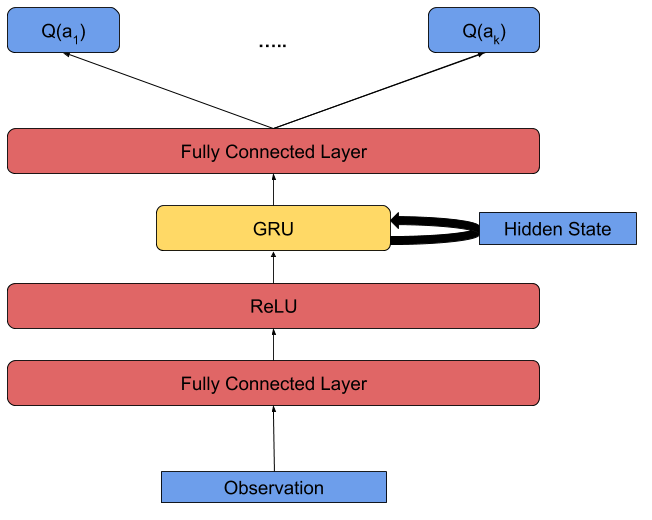
\includegraphics[scale=0.45]{images/agent_diagrams/rnn_agent_diagram.png}
    \caption{The \textbf{RNN} architecture.}
    \label{fig:RNN_agent_diagram}
\end{figure}






\subsection{Grid Representation of Observations and Actions}

A relatively simple way to abstract the observation of a particular agent is to generate a grid (with the agent at the centre) with various channels containing relevant features, with each cell representing a location in this agent's field of view. The features may include whether a particular cell contains an ally or an enemy unit (or neither), the health of a unit and the type of a unit (Marine, Zealot etc.). 

We are also able to represent actions in a similar way. 

In both of these cases, the grids are three dimensional tensors (in the PyTorch framework).

This representation of observations and actions allow for the use of convolutional neural networks to better find patterns in the graphical representation of the environment, as we will explore in the Experiments section. They also provide the first step to making the agent network architecture invariant to the number of units in the scenario.

\subsubsection{Observation and Action Encoders}

Some key pieces of engineering to allow for the use of grid-based observations and actions are the observation encoder and action encoder. 

The observation encoder turns StarCraft II (one dimensional) observations into grid observations. The centre of the grid represents the agent's location, and observations are represented by filling the relevant cell in a specific channel with the necessary observation information, while all other cells have value 0. For example, the health observation sets cells representing unit locations (in the health channel) to the health of those units. 

The action encoder turns StarCraft II actions (one-hot encoding) into grid actions (with 2 channels for movement and attack). In the action grid, the central cell represents the location of the agent. If the action is a movement action, then a 1 is filled in the adjacent north, south, east or west cell (depending on which direction the action is) in the movement channel. All other cells are left as 0. If the action is an attack action, then a 1 is filled in the cell in which the unit to attack is occupying, in the attack channel. Again, all other cells remain as 0. 



Note that both encoders do not have any learned parameters, and are simply used to prepare the inputs before they are passed into the agent network.

\subsubsection{Convolutional Neural Network Architectures}

A possible way to enhance the performance of the simple RNN agent network is to include convolutional layers. This allows the agent network to make stronger deductions about the spatial relations between entities in each observation, and recognise patterns that would otherwise not be noticed, especially when observations and actions are represented as images (grid-based). 

The convolutional layers will form a convolutional encoder, that was originally shown to be successful in \cite{ddpg}, which explored the use of deep deterministic policy gradients (DDPG). The encoder is simply three convolutional layers, which have 32 filters each and no pooling. After each convolutional layer, an exponential linear unit (ELU) is used as the activation function.

Clevert et al. \cite{elu} gave the following advantages of the ELU activation function: ``In contrast to rectified linear units (ReLUs), ELUs can output negative values which allows them to push mean unit activations closer to zero like batch normalisation but with lower computational complexity. Mean shifts toward zero speed up learning by bringing the normal gradient closer to the unit natural gradient because of a reduced bias shift effect.''


We first consider a simple agent network architecture using this convolutional encoder (as well as a GRU-cell). We first feed the grid-based observation into the convolutional encoder, before flattening the output into a 1-dimensional tensor. We do this to be able to concatenate the 1-dimensional observation information (agent ID, last action performed etc.). The next layer is a fully connected linear layer, before a rectified linear unit as the activation function. What follows is a GRU-cell and another fully-connected layer, which outputs a Q-value for each possible action. Intuitively, the convolutional encoder captures various information about the spatial relation between entities in the observation, while the multiple fully-connected layers extract this information to produce the Q-values. The GRU-cell allows for the network to use information about the historical time-series data, to give an even more informed result. We shall refer to this agent network as the \textbf{conv} architecture. This agent network architecture is shown in figure \ref{fig:conv_agent_diagram}.

\begin{figure}
    \centering
    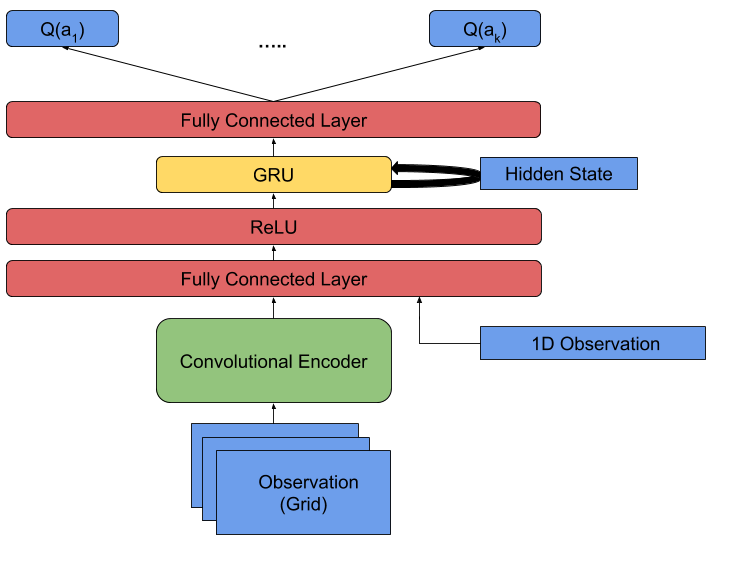
\includegraphics[scale=0.45]{images/agent_diagrams/rnn_conv_dpdpg_agent_diagram.png}
    \caption{The \textbf{conv} architecture.}
    \label{fig:conv_agent_diagram}
\end{figure}

We can also experiment with the idea of using a candidate action as an input in order to output a single Q-value (for that observation-action pair), rather than simply have a Q-value for each possible action. This yields a new agent network architecture, which inputs grid-based observations into the convolutional encoder as normal, but concatenates a candidate action onto the 1-dimensional encoded observation. The layers are the same as in the \textbf{conv} architecture, except that the last fully-connected linear layer has a single output, for the Q-value corresponding to the particular observation and action pair. We shall refer to this agent network architecture as \textbf{conv\_input\_flat}. 

Passing actions as inputs in this way changes the shape of the network, with more neurons at the input (to deal with the action), and less neurons at the output (we no longer output multiple Q-values). This may have implications to the speed of training and overall performance, and is therefore important to experiment with. 

The \textbf{conv\_input\_flat} architecture is shown in figure \ref{fig:conv_input_flat_diagram}.

\begin{figure}
    \centering
    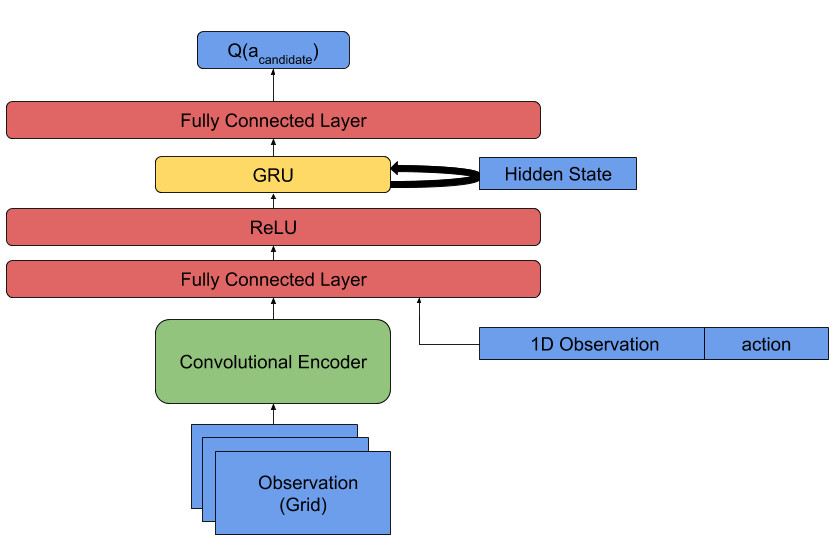
\includegraphics[scale=0.45]{images/agent_diagrams/rnn_mathias_agent_diagram.png}
    \caption{The \textbf{conv\_input\_flat} architecture.}
    \label{fig:conv_input_flat_diagram}
\end{figure}


The previous two architectures’ convolutional encoders do not encode any information about the possible actions, only the observations. Therefore, a possible change that can be made is to somehow include the actions (in their grid-based representations) as an input into the encoder. This requires us to input a particular action into the network first, and receive a single Q-value for that particular observation and action pair, rather than receive a Q-value for each possible action. As described before, actions are represented in a similar way to observations, but with just 2 channels (movement and attack), with a single 1 in a cell to represent movement (or attack) to a particular location in the agent's field of view. The architecture of this agent network is similar to that of the \textbf{conv} architecture, but the action grid representation for a single possible action is concatenated to an observation in its grid representation, and is then fed forward through the network as normal. Therefore, the entire input consists of a series of observation-action pairs (in this concatenated grid form), one for each observation and possible action. We also only have a single output from the last fully connected linear layer, representing the Q-value of that particular observation-action pair. This agent network architecture will be referred to as \textbf{conv\_input\_grid}.

The architecture can be seen in figure \ref{fig:conv_input_grid_agent_diagram}.

\begin{figure}
    \centering
    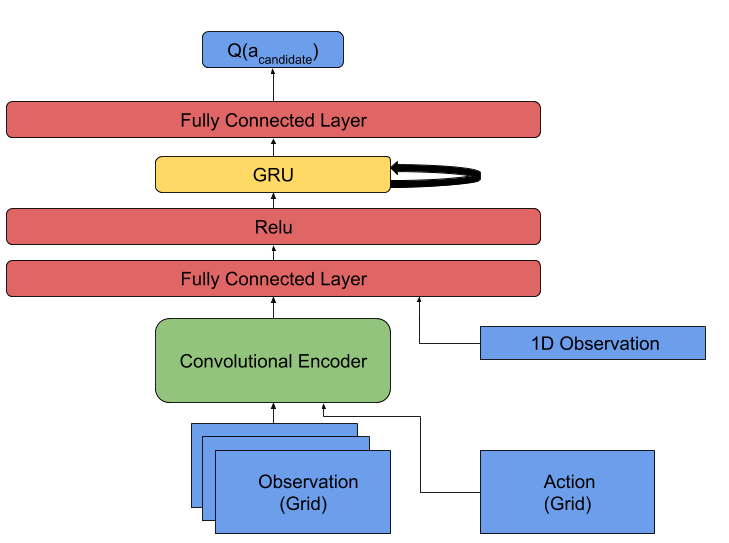
\includegraphics[scale=0.45]{images/agent_diagrams/rnn_conv_ddpg_input_grid_agent_diagram.png}
    \caption{The \textbf{conv\_input\_grid} architecture.}
    \label{fig:conv_input_grid_agent_diagram}
\end{figure}





\subsubsection{Grid Size}

We are able to change the ``resolution'' of the observation (and action) grid by changing its width and height. The grid always covers the field of view of the agent (and no more), but the number of cells in the grid (i.e. the ``resolution'') can be changed.  A larger number of cells in the grid gives a greater number of atomic locations, but also a greater amount of computation will be required and more sparse images will be generated. Therefore, a balance has to be made. This will form a large part of the experiments for these agent network architectures.





\subsection{Problems Encountered}
In the implementation of these agent network architectures, there were multiple challenges to overcome. We briefly overview the most prominent in the following sections.

\subsubsection{Multiple Occupancy}
Observation and available action information can be lost when multiple units are close enough to occupy the same cell in the grid representation, appearing as a single unit to the agent. An agent would be most disadvantaged in cases where the superior actions differ depending on the number of units in a specific location. This is especially apparent with smaller grid resolutions. A simple way to mitigate this effect is to alter the observation to distribute the location of units to neighbouring cells in the case of multiple occupancy. This can be done with a simple randomised algorithm. Algorithm \ref{multipleoccupancyalg} details the procedure.

\begin{algorithm}
    \caption{Resolving Multiple Occupancy (RSO)}
    \label{multipleoccupancyalg}
    \begin{algorithmic}
        \Procedure{ResolveMultipleOccupancy}{}
        \While{there is some cell containing multiple units}
        \State $c$ = a cell with more than one unit
        \State unit = arbitrary unit in cell $c$
        \State $c'$ = random cell adjacent to $c$
        \State move unit from $c$ to $c'$
        \EndWhile
        
        \EndProcedure
      
        
        
    \end{algorithmic}
    
\end{algorithm}

\subsubsection{Memory Usage}

Memory usage was large for the architectures using a grid representation of observations or actions, especially on maps with more than 10 units. This can be explained by the sparsity of the grid tensors: there are only $n$ cells with non-zero values, where $n$ is the total number of units in the map, compared to a total of $W \times H \times C$ cells ($W$, $H$, $C$ being the width, height and number of channels in the grid respectively). Each cell is a 4-byte float, thus a single grid representation of observations and actions (of size $12 \times 12$, and with 3 observation channels and 2 action channels) uses $4 \times 12 \times 12 \times 5 = 2880$ bytes. 

The replay buffer contains the most recent 5000 episodes, with each episode estimated to being at least 100 timesteps. We have an observation for each agent and each available action, so in a map with 3 agents and 9 available actions there are at least $5000 \times 100 \times 3 \times 9 = 1.35 \times 10^7$ such grids in the replay buffer. This gives a minimum total size of $1.35 \times 10^7 * 2880 \text{ bytes} \approx 38.9$GB, which is far too large for RAM, let alone GPU memory.


A solution to this problem is to use a compressed representation: storing the observations and actions as lists in the buffer, and decompressing them into the grid representation ``on-the-fly''. This method proved successful and allowed the replay buffer to be stored easily in RAM, albeit with a computation time trade-off.

However, on larger grid sizes (e.g $24\times24$) the batch was still too larger. A standard batch size of 32 \cite{smac} gives an average total size of at least $500$MB, but this can easily become too large for the GPU memory. 

A smaller batch size is therefore used for larger grid sizes (above $12 \times 12$). However, the batch size can have an effect on training performance: a larger batch size generally decreases the variance of the estimates of Q-values, allowing for more consistent gradient descent traversals. However, a lower batch size can introduce more noise in the sampling, and allows for escaping local minima, as well as avoiding overfitting.

With these considerations, in situations where memory usage is high, it is generally advisable for the batch size to be as large as possible before memory usage becomes too high \cite{batchsizes}. Testing found the following batch sizes effective with a 6GB GPU memory limit for various grid sizes.

\vspace{3mm}
\begin{center}
\begin{tabular}{ |p{1.8cm}||p{1.8cm}|p{8cm}|  }
 \hline
 Grid Size& batch\_size& Approximate Memory Usage During Training (GB)\\
 \hline
 \centering 6x6   & \centering 32 & \centering2.0\tabularnewline
 \hline \centering 12x12   & \centering 32 & \centering4.5\tabularnewline
 \hline
 \centering 18x18   & \centering 16 & \centering5.0\tabularnewline
 \hline
 \centering 24x24   & \centering12 & \centering5.5\tabularnewline
 \hline
\end{tabular}
\end{center}
\vspace{3mm}












\subsection{StarCraft Task Invariant Architectures}
Architectures that use actions or agent IDs (in their standard representations) as inputs or outputs are not invariant to the task in StarCraft II. This is because a different map may have a different number of units, and thus a different number of enemies to attack and more agent IDs to assign. This requires a larger one-hot encoding, so the architecture is changed. This section explains an attempt to remove this dependence on the scenario.


Grid-representation of observations and actions get us closer to this invariance, as actions are no longer one-hot encoded, but are represented in a universal grid form. Furthermore, this representation is well-suited to generalising over tasks as agent interactions depend on spatial arrangement. 

The architecture closest to task invariance is \textbf{conv\_input\_grid}, since it uses grid observations and actions. Furthermore, in order to make it fully invariant to tasks, we simply need to remove the input for the agent ID and use the VDN mixing network (QMIX requires an input for each agent, so is not invariant, but the VDN network does not have this problem as it is simply a sum of Q-values). In Section 4, we experiment with the removal of the agent ID as an input, allowing us to evaluate its necessity.  


Therefore, by removing this input from the \textbf{conv\_input\_grid} architecture, we produce our final architecture, \textbf{conv\_input\_grid\_no\_id}, which (when used with the VDN mixing network) is task invariant.




A huge advantage to network architectures which are invariant to the task is the ability for transfer learning. Due to the similarity of the tasks (a consequence of partial observability), it may be useful to train on smaller, simpler tasks before attempting to learn on more complex tasks with a far greater state space. This has shown to have the effect of speeding up training time and even increasing final performance \cite{curriculum}.



